\documentclass[12pt,a4paper]{article}
\usepackage{graphicx, booktabs, siunitx, amsmath, geometry, float}
\usepackage{subcaption}
\geometry{margin=2.5cm}
\title{M1 & M2: Investigation of Transistor Amplifiers}
\author{Gregorio Jaca U8L9B9, Peter Tallosy K14WR1 }
\date{\today}

\begin{document}
%\maketitle

\section{M1: Investigation of a Common-Emitter Amplifier}

\subsection{DC Operating Point}
The DC voltages of the amplifier were measured at the transistor's electrodes with the input left open.
\begin{itemize}
    \item $U_B = \SI{1.28}{V}$
    \item $U_C = \SI{6.96}{V}$
    \item $U_E = \SI{0.66}{V}$
\end{itemize}
From these, the base-emitter and collector-emitter voltages were calculated:
\begin{itemize}
    \item $U_{BE} = U_B - U_E = \SI{0.62}{V}$
    \item $U_{CE} = U_C - U_E = \SI{6.3}{V}$
\end{itemize}

The $U_{BE}$ value is within the range of typical value for a silicon transistor, between 0.6 and 0.7 V. Considering the supply voltage of 15 V (The effective supply voltage would be the supply voltage minus the voltage dropped on the protective diode) the value for $U_{CE}$ is very close to the ideal mid-point value. This indicates a good operational point.

\subsection{Saturation Measurement}
A \SI{1}{kHz} sinusoidal input signal was applied. The input amplitude was increased until the output signal began to show distortion. Saturation was observed to begin at an input amplitude of \SI{150}{mV}. A phase shift of approximately 180° was produced. 

\begin{figure}[H]
    \centering
    \begin{subfigure}[b]{0.48\linewidth}
        \centering
        \includegraphics[width=\linewidth]{unsaturated.png}
    \end{subfigure}\hfill
    \begin{subfigure}[b]{0.48\linewidth}
        \centering
        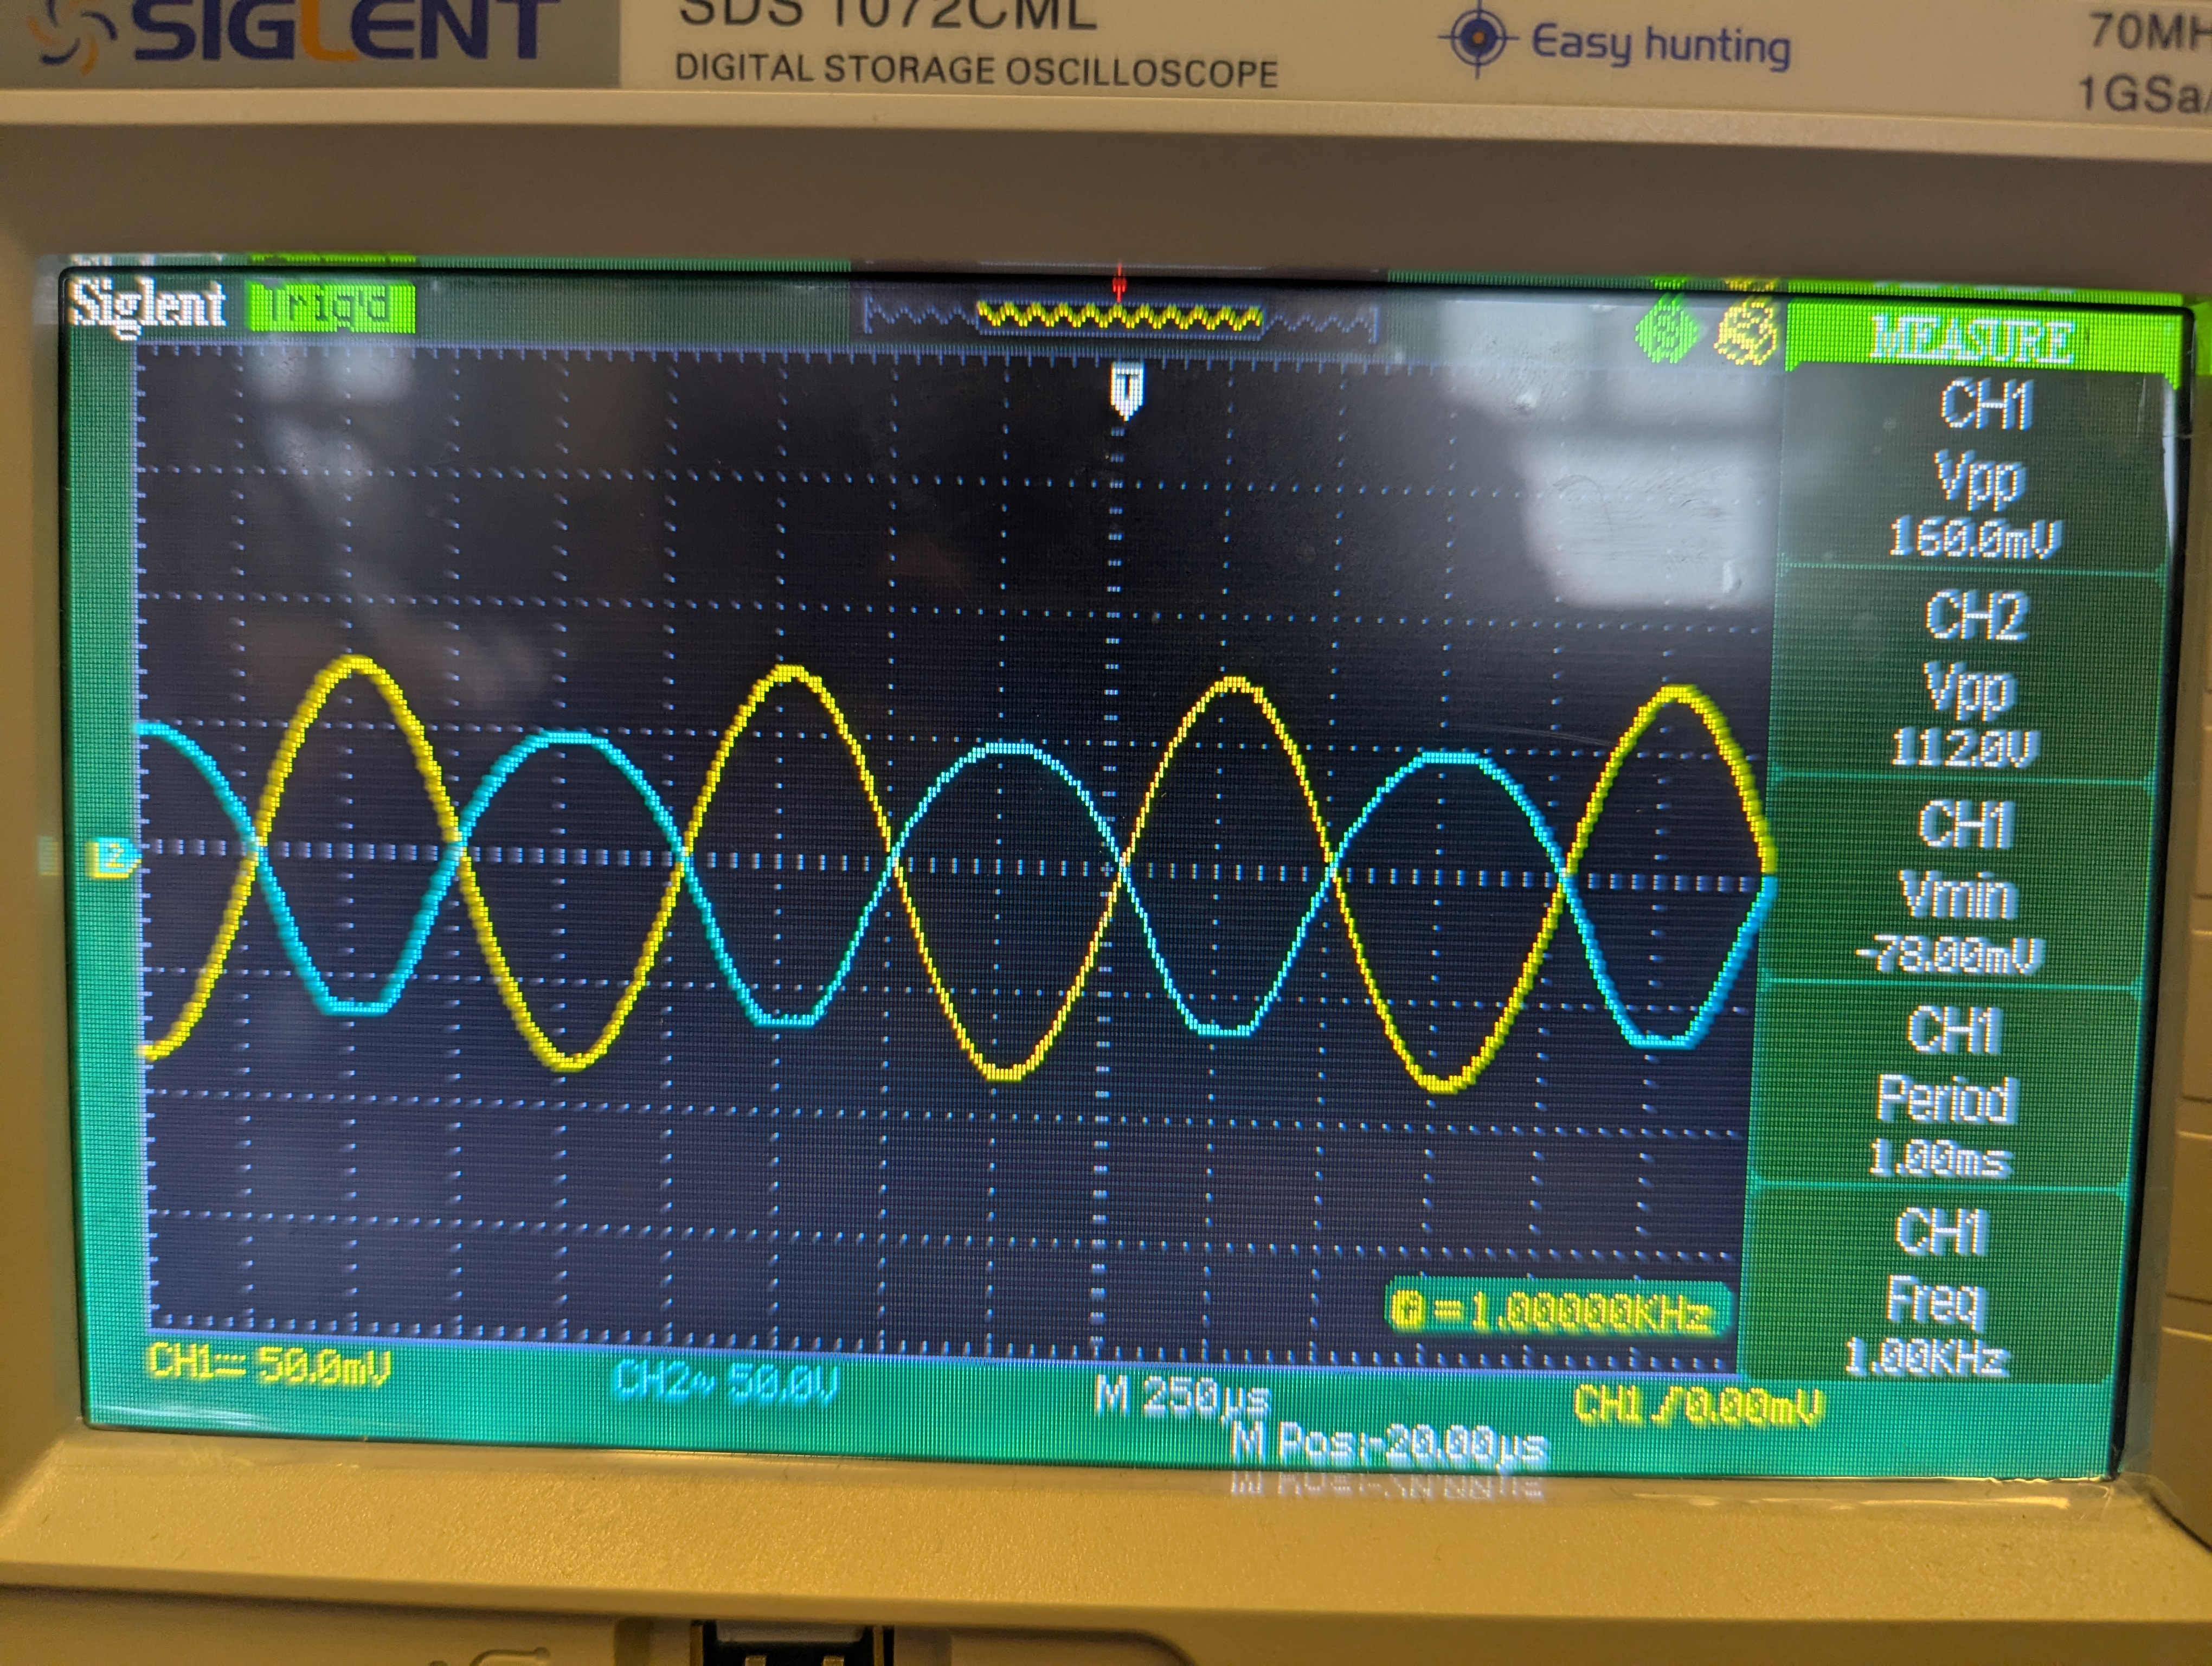
\includegraphics[width=\linewidth]{saturated_160mv.jpg.png}
    \end{subfigure}
    \caption{Amplifier output at the oscillator. Left: 100mV, unsaturated , Right: 160mV saturated at the negative voltages.}
    \label{fig:oscilloscope}
\end{figure}

Looking at the oscilloscope, we noticed that the signal saturated first at the negative voltages. This asymmetry initially suggests that the Q-point, the DC operating point is too high. We know, and it can be seen in Fig. \ref{fig:oscilloscope}, that the common emitter amplifier inverts the voltage sign. Therefore, the fact that the negative voltages \textbf{at the output} saturate means that the positive input (including the bias voltage) is too high. However, in the previous section we measured the DC operational point and saw that the Q-point was not high, if anything, it was slightly below the mid-point. Therefore, the above explanation is unsatisfactory. Other posibilities which we considered, but could not test, are: transistor non-linearity and gain variation, and input and output capacitor effects. 


\subsection{Frequency Response}
The frequency response of the amplifier was measured by applying a sinusoidal input of constant amplitude and varying the frequency. The input and output voltages were recorded at several frequencies.

\begin{table}[H]
    \centering
    \caption{Frequency response data for Common-Emitter amplifier (M1.c).}
    \label{tab:freq_response_m1}
    \sisetup{table-format=3.2}
    \begin{tabular}{lccccccccccc}
        \toprule
        {$f$ (\si{Hz})} & 50 & 100 & 200 & 500 & 1k & 2k & 5k & 10k & 20k & 50k & 100k \\
        \midrule
        {$U_{in}$ (\si{mV})} & 120 & 118 & 112 & 112 & 110 & 110 & 112 & 112 & 110 & 110 & 112 \\
        {$U_{out}$ (\si{mV})} & 4800 & 6400 & 7200 & 7400 & 7400 & 7400 & 7400 & 7400 & 7200 & 6200 & 4800 \\
        {$A_u$} & 40.00 & 54.24 & 64.29 & 66.07 & 67.27 & 67.27 & 66.07 & 66.07 & 65.45 & 56.36 & 42.86 \\
        {$a_u$ (\si{dB})} & 32.04 & 34.69 & 36.16 & 36.40 & 36.56 & 36.56 & 36.40 & 36.40 & 36.32 & 35.02 & 32.64 \\
        {$\phi$ (\si{\degree})} & 108 & 134 & 147 & 160 & 164 & 166 & 170 & 178 & 187 & 208 & 225 \\
        \bottomrule
    \end{tabular}
\end{table}

% \begin{figure}[H]
%     \centering
%     % GGG: Create Bode plot (au vs f) and phase plot (phi vs f) from the table data for M1.
%     \includegraphics[width=0.7\linewidth]{bode_plot_m1.png}
%     \caption{}
%     \label{fig:bode_plot_m1}
% \end{figure}



\begin{figure}[H]
    \centering
    \begin{subfigure}[b]{0.48\linewidth}
        \centering
        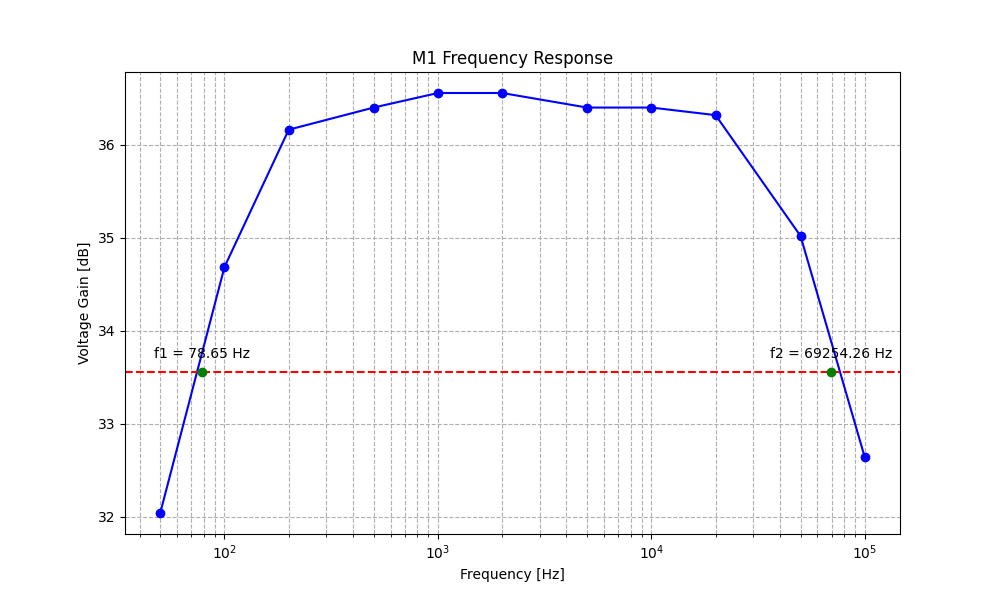
\includegraphics[width=\linewidth]{m1_frequency_response.png}
    \end{subfigure}\hfill
    \begin{subfigure}[b]{0.48\linewidth}
        \centering
        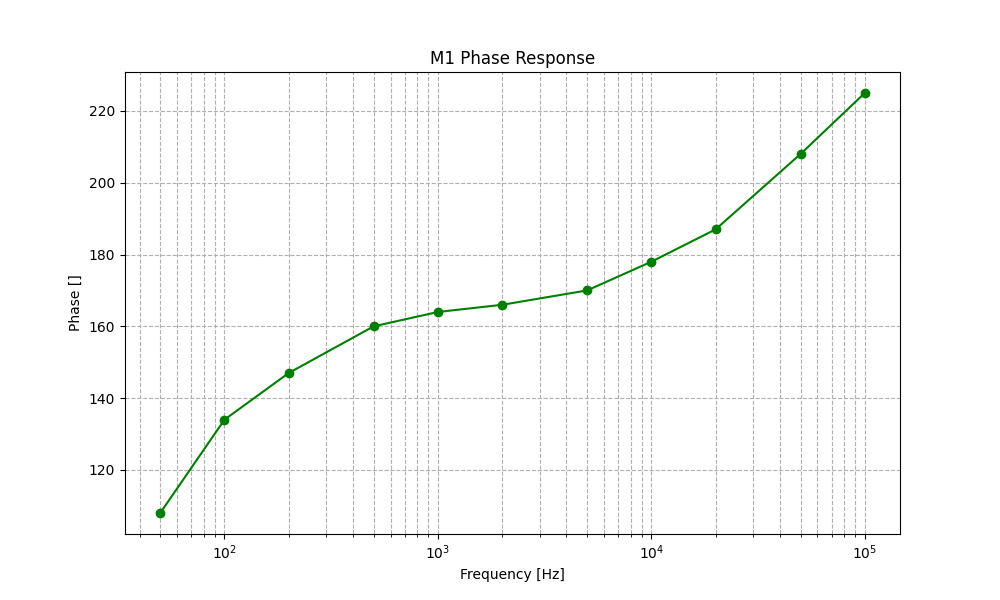
\includegraphics[width=\linewidth]{m1_phase_response.png}
    \end{subfigure}
    \caption{Bode plot of the common-emitter amplifier's frequency response. Left: Amplification , Right: Phase}
    \label{fig:bode_plot_m1}
\end{figure}

From the frequency response characteristics we can identify the upper and lower cut-offs: $f_l = \SI{78.6}{Hz}$ and $f_u = \SI{69.3}{kHz}$. The bandwidth of the amplifier is $B = f_u - f_l = \SI{69.2}{kHz}$. 

\subsection{Miller Effect}
A \SI{22}{pF} capacitor was connected between the collector and base of the transistor. This reduced the upper cut-off frequency to $f_u = \SI{12}{kHz}$, and did not modify the low frequency characteristics. This is expected as the capacitor's impeadance increases with the frequency. This shows the importance of reducing the capacitance between the electrodes in a circuit.

\subsection{Cascade Circuit}
The circuit was modified into a cascade configuration. This increased the upper cut-off frequency significantly to $f_u = \SI{271}{kHz}$.

\section{M2: Investigation of a Common-Collector Amplifier}

\subsection{Gain and Phase Shift}
At \SI{1}{kHz}, with an input of $U_{in} = \SI{1}{V}$, the output was $U_{out} = \SI{980}{mV}$. This gives a voltage gain of $A_u = 0.98$. The phase shift was $\phi = \SI{0}{\degree}$. This is typical of common collector amplifiers which have a close to unity voltage gain.

\subsection{Frequency Response}
The frequency response was investigated at several input frequencies.

\begin{table}[H]
    \centering
    \caption{Frequency response data for Common-Collector amplifier (M2.b).}
    \label{tab:freq_response_m2}
    \sisetup{table-format=1.3}
    \begin{tabular}{lccccc}
        \toprule
        {$f$ (\si{Hz})} & 100 & 1k & 10k & 100k & 1000000 \\
        \midrule
        {$U_{in}$ (\si{mV})} & 1050 & 1010 & 1010 & 1010 & 1000 \\
        {$U_{out}$ (\si{mV})} & 960 & 920 & 920 & 928 & 928 \\
        {$A_u$} & 0.914 & 0.911 & 0.911 & 0.919 & 0.928 \\
        {$a_u$ (\si{dB})} & -0.78 & -0.81 & -0.81 & -0.74 & -0.65 \\
        {$\phi$ (\si{\degree})} & 0.0 & 0.2 & 0.0 & 0.0 & 7.2 \\
        \bottomrule
    \end{tabular}
\end{table}

\begin{figure}[H]
    \centering
    \begin{subfigure}[b]{0.48\linewidth}
        \centering
        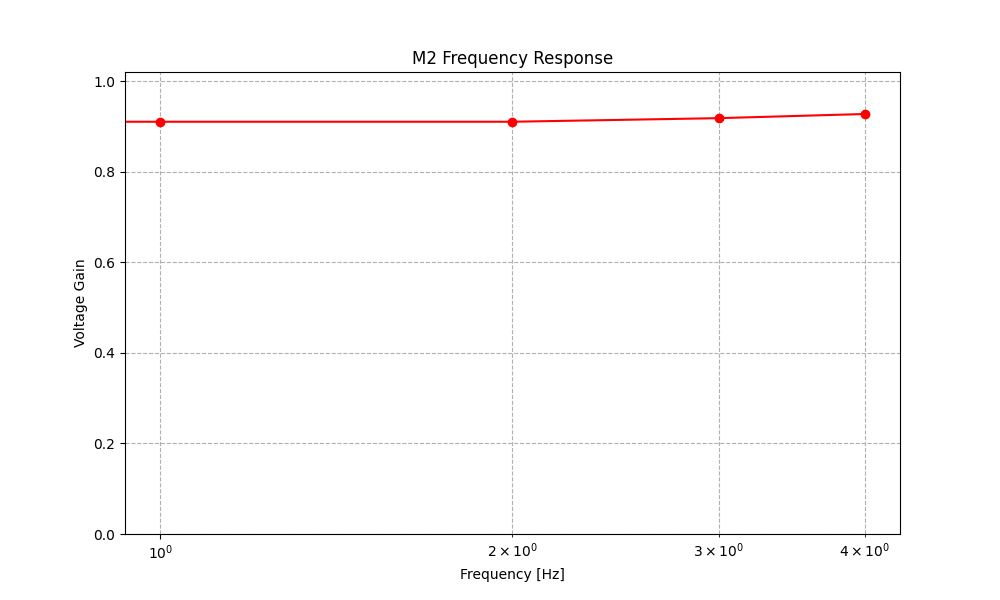
\includegraphics[width=\linewidth]{m2_frequency_response_A.png}
    \end{subfigure}\hfill
    \begin{subfigure}[b]{0.48\linewidth}
        \centering
        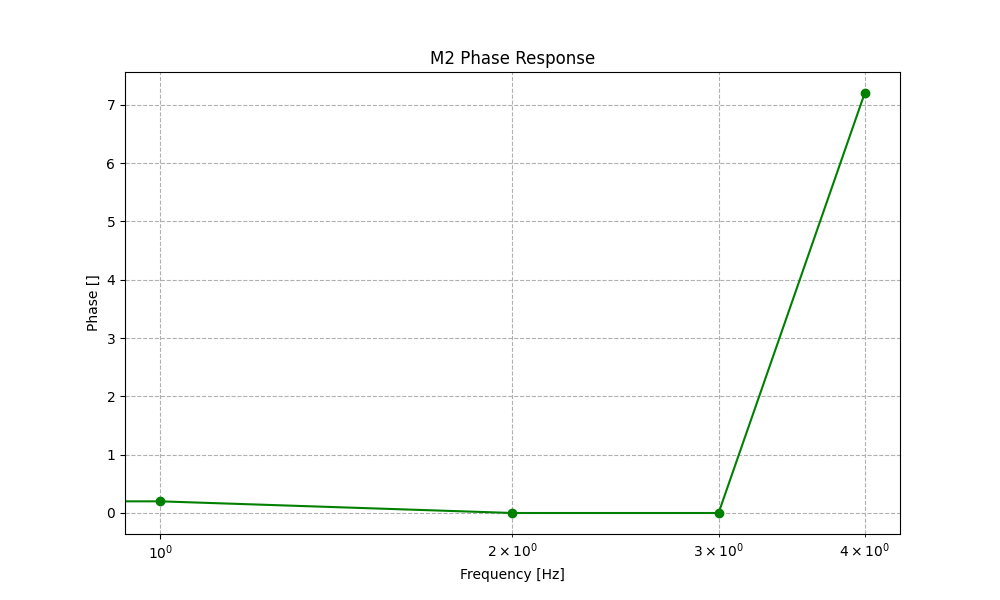
\includegraphics[width=\linewidth]{m2_phase_response.png}
    \end{subfigure}
    \caption{Bode plot of the common-collector amplifier's frequency response. Left: Amplification , Right: Phase}
    \label{fig:bode_plot_m2}
\end{figure}

As expected, the voltage gain is smaller but close to unity

\subsection{Input Resistance}
The input resistance of the common-collector amplifier was measured to be $R_{in} = \SI{37.4}{k\ohm}$.

\subsection{High Input Resistance Configuration}
The circuit was modified to a high input resistance configuration. The input resistance was measured to be $R_{in} = \SI{248}{k\ohm}$.

\section{Conclusion}
The characteristics of a common-emitter amplifier were measured. The operating point, gain, and bandwidth were determined. The measurements confirm the expected behavior, including the \SI{180}{\degree} phase inversion and the frequency limitations of the amplifier. The Miller effect and the cascade configuration demonstrated methods to influence the high-frequency performance.

The common-collector amplifier was also investigated, confirming its characteristics such as voltage gain close to unity, no phase inversion, and high input impedance.

\end{document}

% GGG
We did not properly save the table data during our measurement excercise and we lost it. Czehlár Gergely and Hunyady Csongor were kind enough to share this data with us. The raw data in Tables 1 and 2 \ref{\ref{tab:freq_response_m1}} and \ref{\ref{tab:freq_response_m2}} is theirs.